\documentclass[border=5pt]{standalone}
\usepackage{tikz}
\usepackage{amsmath}
\begin{document}
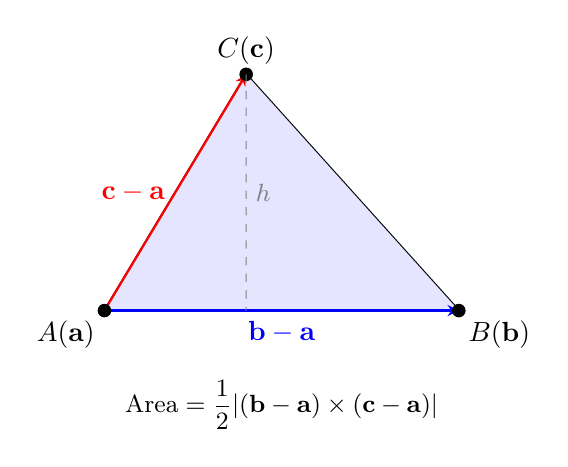
\begin{tikzpicture}[scale=1.5, >=stealth]
  % Triangle with vertices A, B, C
  \coordinate (A) at (0,0);
  \coordinate (B) at (3,0);
  \coordinate (C) at (1.2,2);

  % Triangle
  \draw[thick] (A) -- (B) -- (C) -- cycle;

  % Fill with light color
  \fill[blue!10] (A) -- (B) -- (C) -- cycle;

  % Vectors
  \draw[->, thick, blue] (A) -- (B) node[midway, below] {$\mathbf{b}-\mathbf{a}$};
  \draw[->, thick, red] (A) -- (C) node[midway, left] {$\mathbf{c}-\mathbf{a}$};

  % Vertices
  \filldraw[black] (A) circle (1.5pt) node[below left] {$A(\mathbf{a})$};
  \filldraw[black] (B) circle (1.5pt) node[below right] {$B(\mathbf{b})$};
  \filldraw[black] (C) circle (1.5pt) node[above] {$C(\mathbf{c})$};

  % Height
  \draw[dashed, gray, thin] (C) -- (1.2, 0);
  \node[right, font=\small, gray] at (1.2, 1) {$h$};

  % Area formula
  \node[font=\small] at (1.5, -0.8) {$\text{Area} = \dfrac{1}{2}|(\mathbf{b}-\mathbf{a})\times(\mathbf{c}-\mathbf{a})|$};
\end{tikzpicture}
\end{document}
